\documentclass{standalone}
\usepackage{tikz}
\usetikzlibrary{shapes.geometric}
\begin{document}
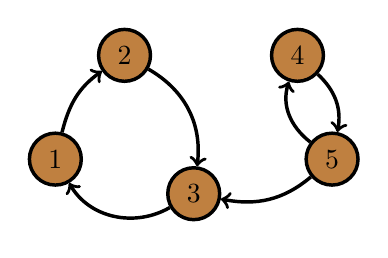
\begin{tikzpicture}
[every node/.style={inner sep=0pt}]
\node (1) [circle, minimum size=18.75pt, fill=brown, line width=1.25pt, draw=black] at (25.0pt, -75.0pt) {\textcolor{black}{1}};
\node (2) [circle, minimum size=18.75pt, fill=brown, line width=1.25pt, draw=black] at (50.0pt, -37.5pt) {\textcolor{black}{2}};
\node (4) [circle, minimum size=18.75pt, fill=brown, line width=1.25pt, draw=black] at (112.5pt, -37.5pt) {\textcolor{black}{4}};
\node (5) [circle, minimum size=18.75pt, fill=brown, line width=1.25pt, draw=black] at (125.0pt, -75.0pt) {\textcolor{black}{5}};
\node (3) [circle, minimum size=18.75pt, fill=brown, line width=1.25pt, draw=black] at (75.0pt, -87.5pt) {\textcolor{black}{3}};
\draw [line width=1.25, ->, color=black] (1) to  [in=215, out=76] (2);
\draw [line width=1.25, ->, color=black] (2) to  [in=83, out=330] (3);
\draw [line width=1.25, ->, color=black] (3) to  [in=300, out=210] (1);
\draw [line width=1.25, ->, color=black] (5) to  [in=349, out=220] (3);
\draw [line width=1.25, ->, color=black] (5) to  [in=252, out=142] (4);
\draw [line width=1.25, ->, color=black] (4) to  [in=79, out=317] (5);
\end{tikzpicture}

\end{document}
